
\documentclass[ignorenonframetext, compress, 9pt, xcolor=svgnames]{beamer} 
\usepackage{pdfpages}
\usepackage{amsmath}
\usepackage{amsfonts}
\usepackage{amssymb}
\setbeamercolor{frametitle}{fg=DarkBlue}
\setbeamercolor{sectionpage title}{bg=DarkBlue}
%\setbeamercolor{section in head/foot}{bg=DarkBlue}
%\setbeamercolor{author in head/foot}{bg=DarkBlue}
\setbeamercolor{author in head/foot}{fg=DarkBlue}
%\setbeamercolor{title in head/foot}{bg=White}
\setbeamercolor{title in head/foot}{fg=DarkBlue}
%\setbeamercolor{date in head/foot}{fg=Brown}
%\setbeamercolor{alerted text}{fg=DarkBlue}
%\usecolortheme[named=DarkBlue]{structure} 
%\usepackage{bbm}
%\usepackage{bbold}
\usepackage{eurosym}
\usepackage{graphicx}
%\usepackage{epstopdf}
\usepackage{hyperref}
\hypersetup{
  colorlinks   = true, %Colours links instead of ugly boxes
  urlcolor     = DarkBlue, %Colour for external hyperlinks
  linkcolor    = DarkBlue, %Colour of internal links
  citecolor   = DarkRed %Colour of citations
}
\usepackage{multirow}
\usepackage{xspace}
\usepackage{listings}
\usepackage{natbib}
\usepackage{booktabs}
\usepackage{dcolumn}
\usepackage[greek,frenchb]{babel}
\usepackage[utf8]{inputenc}
\usepackage[T1]{fontenc}
\usepackage{natbib}
\renewcommand{\cite}{\citet}
\usepackage{longtable}
\setbeamertemplate{caption}[numbered]
\setbeamertemplate{theorem}[ams style]
\setbeamertemplate{theorems}[numbered]
%\usefonttheme{serif}
%\usecolortheme{beaver}
%\usetheme{Hannover}
%\usetheme{CambridgeUS}
%\usetheme{Madrid}
%\usecolortheme{whale}
%\usetheme{Warsaw}
%\usetheme{Luebeck}
\usetheme{Montpellier}
%\usetheme{Berlin}
%\setbeamercolor{titlelike}{parent=structure}
%\setbeamertemplate{headline}[default]
%\setbeamertemplate{footline}[default]
%\setbeamertemplate{footline}[Malmoe]
%\setbeamercovered{transparent}
%\setbeamercovered{invisible}
%\usecolortheme{crane}
%\usecolortheme{dolphin}
%\usepackage{pxfonts}
%\usepackage{isomath}
%\usepackage{mathpazo}
%\usepackage{arev} %     (Arev/Vera Sans)
%\usepackage{eulervm} %_   (Euler Math)
%\usepackage{fixmath} %  (Computer Modern)
%\usepackage{hvmath} %_   (HV-Math/Helvetica)
%\usepackage{tmmath} %_   (TM-Math/Times)
%\usepackage{tgheros}
%\usepackage{cmbright}
%\usepackage{ccfonts} \usepackage[T1]{fontenc}
%\usepackage[garamond]{mathdesign}

%\usepackage{color}
%\usepackage{ulem}

%\usepackage[math]{kurier}
%\usepackage[no-math]{fontspec}
%\setmainfont{Fontin Sans}
%\setsansfont{Fontin Sans}
%\setbeamerfont{frametitle}{size=\LARGE,series=\bfseries}

% suppress navigation bar
\beamertemplatenavigationsymbolsempty
%\usetheme{bunsenMod}
%\setbeamercovered{transparent}
%\setbeamertemplate{items}[circle]
%\usecolortheme[named=CadetBlue]{structure}
%\usecolortheme[RGB={225,64,5}]{structure}
%\definecolor{burntRed}{RGB}{225,64,5}
%\setbeamercolor{alerted text}{fg=burntRed} 
%\usecolortheme[RGB={0,40,110}]{structure}
%\hypersetup{linkcolor=burntRed}
%\hypersetup{urlcolor=burntRed}
%\hypersetup{filecolor=burntRed}
%\hypersetup{citecolor=burntRed}

%\usetheme{bunsenMod}
%\setbeamercovered{transparent}
%\setbeamertemplate{items}[circle]
%\usecolortheme[named=CadetBlue]{structure}
%\usecolortheme[RGB={225,64,5}]{structure}
%\definecolor{burntRed}{RGB}{225,64,5}
%\setbeamercolor{alerted text}{fg=burntRed} 
%\usecolortheme[RGB={0,40,110}]{structure}
%\hypersetup{linkcolor=burntRed}
%\hypersetup{urlcolor=burntRed}
%\hypersetup{filecolor=burntRed}
%\hypersetup{citecolor=burntRed}

%\AtBeginSection[] % Do nothing for \section*
%{ \frame{\sectionpage} }
%\setbeamertemplate{frametitle continuation}{}
\newtheorem{lemme}{Lemme}[section]
\newtheorem{remarque}{Remarque}
\newcommand{\argmax}{\operatornamewithlimits{arg\,max}}
\newcommand{\argmin}{\operatornamewithlimits{arg\,min}}
\def\inprobLOW{\rightarrow_p}
\def\inprobHIGH{\,{\buildrel p \over \rightarrow}\,} 
\def\inprob{\,{\inprobHIGH}\,} 
\def\indist{\,{\buildrel d \over \rightarrow}\,} 
\def\sima{\,{\buildrel a \over \sim}\,} 
\def\F{\mathbb{F}}
\def\R{\mathbb{R}}
\newcommand{\gmatrix}[1]{\begin{pmatrix} {#1}_{11} & \cdots &
    {#1}_{1n} \\ \vdots & \ddots & \vdots \\ {#1}_{m1} & \cdots &
    {#1}_{mn} \end{pmatrix}}
\newcommand{\iprod}[2]{\left\langle {#1} , {#2} \right\rangle}
\newcommand{\norm}[1]{\left\Vert {#1} \right\Vert}
\newcommand{\abs}[1]{\left\vert {#1} \right\vert}
\renewcommand{\det}{\mathrm{det}}
\newcommand{\rank}{\mathrm{rank}}
\newcommand{\spn}{\mathrm{span}}
\newcommand{\row}{\mathrm{Row}}
\newcommand{\col}{\mathrm{Col}}
\renewcommand{\dim}{\mathrm{dim}}
\newcommand{\prefeq}{\succeq}
\newcommand{\pref}{\succ}
\newcommand{\seq}[1]{\{{#1}_n \}_{n=1}^\infty }
\renewcommand{\to}{{\rightarrow}}
\renewcommand{\L}{{\mathcal{L}}}
\newcommand{\Er}{\mathrm{E}}
\renewcommand{\Pr}{\mathrm{P}}
%\newcommand{\Var}{\mathrm{Var}}
%\newcommand{\Cov}{\mathrm{Cov}}
\newcommand{\corr}{\mathrm{Corr}}
%\newcommand{\Var}{\mathrm{Var}}
\newcommand{\bias}{\mathrm{Bias}}
\newcommand{\mse}{\mathrm{MSE}}
\providecommand{\Pred}{\mathcal{P}}
\providecommand{\plim}{\operatornamewithlimits{plim}}
\providecommand{\avg}{\frac{1}{n} \underset{i=1}{\overset{n}{\sum}}}
\providecommand{\sumin}{{\sum_{i=1}^n}}
\providecommand{\limp}{\overset{p}{\longrightarrow}}
\providecommand{\limp}{\underset{n \rightarrow \infty}{\overset{p}{\longrightarrow}}}
%\providecommand{\limp}{\underset{n \rightarrow \infty}{\overset{p}{\longrightarrow}}}
\providecommand{\limp}{\overset{p}{\longrightarrow}}
%\providecommand{\limd}{\underset{n \rightarrow \infty}{\overset{d}{\longrightarrow}}}
\providecommand{\limd}{\overset{d}{\longrightarrow}}
\def\independenT#1#2{\mathrel{\setbox0\hbox{$#1#2$}%
    \copy0\kern-\wd0\mkern4mu\box0}} 
\newcommand\indep{\protect\mathpalette{\protect\independenT}{\perp}}


\lstset{language=R}
\lstset{keywordstyle=\color[rgb]{0,0,1},                                        % keywords
        commentstyle=\color[rgb]{0.133,0.545,0.133},    % comments
        stringstyle=\color[rgb]{0.627,0.126,0.941}      % strings
}       
\lstset{
  showstringspaces=false,       % not emphasize spaces in strings 
  columns=fixed,
  numbersep=3mm, numbers=left, numberstyle=\tiny,       % number style
  frame=none,
  framexleftmargin=5mm, xleftmargin=5mm         % tweak margins
}
\makeatletter
%\setbeamertemplate{frametitle continuation}{\gdef\beamer@frametitle{}}
\setbeamertemplate{frametitle continuation}{\frametitle{}}
\makeatother

\newtheorem{theoreme}{Théorème}
\newtheorem{proposition}{Proposition}
\newtheorem{corollaire}{Corollaire}
\newtheorem{exemple}{Exemple}
\newtheorem{assumption}{Assumption}
\renewcommand{\theassumption}{A\arabic{assumption}}
\newtheorem{hypothese}{Hypothèse}
\renewcommand{\thehypothese}{H\arabic{hypothese}}
%\newcommand{\Var}{\mathbb{V}}
\newcommand{\Var}{\mathrm{Var}}
\renewcommand{\Er}{\mathbb{E}}
\newcommand{\LP}{\mathcal{LP}}
\providecommand{\Id}{\mathbf{I}}
\providecommand{\Rang}{\mathrm{Rang}}
\providecommand{\Trace}{\mathrm{Trace}}
%\renewcommand{\Cov}{\mathbb{C}}
\newcommand{\Cov}{\mathrm{Cov}}
\providecommand{\Corr}{\mathrm{Corr}}
\providecommand{\Diag}{\mathrm{Diag}}
\providecommand{\reg}{\mathrm{r}}
\providecommand{\Likelihood}{\mathrm{L}}
\renewcommand{\Pr}{{\mathbb{P}}}
\providecommand{\set}[1]{\left\{#1\right\}}
\providecommand{\uvec}{\mathbf{1}}
\providecommand{\Rang}{\mathrm{Rang}}
\providecommand{\Trace}{\mathrm{Trace}}
\providecommand{\Tr}{\mathrm{Tr}}
\providecommand{\CI}{\mathrm{CI}}
\providecommand{\asyvar}{\mathrm{AsyVar}}
\newcommand{\inputslide}[2]{{
    \usebackgroundtemplate{
      \includegraphics[page={#2},width=\paperwidth,keepaspectratio=true]
      {{#1}}}
    \frame[plain]{}
  }}
\newcommand\pperp{\perp\!\!\!\perp}
\usepackage{bbm}
\providecommand{\Ind}{\mathbf{1}}
\newcommand{\sumjsi}{\underset{i<j}{{\sum}}}
\newcommand{\prodjsi}{\underset{i<j}{{\prod}}}
\newcommand{\sumisj}{\underset{j<i}{{\sum}}}
\newcommand{\prodisj}{\underset{j<i}{{\prod}}}
\newcommand{\sumobs}{\underset{i=1}{\overset{N}{\sum}}}
\newcommand{\prodobs}{\underset{i=1}{\overset{N}{\prod}}}
%\newcommand{\sumobs}{\sum_{i=1}^N}
%\newcommand{\prodobs}{\prod_{i=1}^N}
%\newcommand{\sumjsi}{\sum_{i<j}}
%\newcommand{\prodjsi}{\prod_{i<j}}
%\newcommand{\sumisj}{\sum_{j<i}}
%\newcommand{\prodisj}{\sum_{j<i}}

\usepackage{appendixnumberbeamer}
\setbeamertemplate{footline}[frame number]
\setbeamertemplate{section in toc}[sections numbered]
\setbeamertemplate{subsection in toc}[subsections numbered]
\setbeamertemplate{subsubsection in toc}[subsubsections numbered]

\makeatother
\setbeamertemplate{footline}
{
    \leavevmode%
    \hbox{%
        \begin{beamercolorbox}[wd=.333333\paperwidth,ht=2.25ex,dp=1ex,center]{author in head/foot}%
            \usebeamerfont{author in head/foot}\insertshortauthor
        \end{beamercolorbox}%
        \begin{beamercolorbox}[wd=.333333\paperwidth,ht=2.25ex,dp=1ex,center]{title in head/foot}%
            \usebeamerfont{title in head/foot}\insertshorttitle
        \end{beamercolorbox}%
        \begin{beamercolorbox}[wd=.333333\paperwidth,ht=2.25ex,dp=1ex,right]{date in head/foot}%
            \usebeamerfont{date in head/foot}\insertshortdate{}\hspace*{2em}
            \insertframenumber{} / \inserttotalframenumber\hspace*{2ex} 
        \end{beamercolorbox}}%
        \vskip0pt%
    }
    \makeatother
\setbeamertemplate{navigation symbols}{}
\setbeamertemplate{itemize items}[square]

 \usepackage{eso-pic}
\newcommand\AtPagemyUpperLeft[1]{\AtPageLowerLeft{%
\put(\LenToUnit{0.9\paperwidth},\LenToUnit{0.9\paperheight}){#1}}}
\AddToShipoutPictureFG{
  \AtPagemyUpperLeft{{
\includegraphics[width=1.1cm,keepaspectratio]{../logo-uga.png}}}
}%

\title[Econometrics 1: Regression]{UGA M1: Econometrics 1\\
  \textbf{Introduction to Regression}}
\date{\today}
\author{Michal W. Urdanivia\inst{*}}
\institute{\inst{*}Universit\'e de Grenoble Alpes, Facult\'e d'\'Economie, GAEL, \\e-mail: \href{mailto:michal.wong-urdanivia@univ-grenoble-alpes.fr}{michal.wong-urdanivia@univ-grenoble-alpes.fr}}


\begin{document}

\frame{\titlepage}
%\setcounter{tocdepth}{2}



\part{Definition and interpretation of regression}
\frame{\partpage}
\begin{frame}
  \tableofcontents  
\end{frame}

\begin{frame}[allowframebreaks]
  \frametitle{References}
  \begin{itemize}
  \item \cite{ap2014} chapter 2
  \item \cite{w2013} chapter 2    
  \item \cite{sw2009} chapter 4-5
  %\item These slides draw heavily from \cite{angrist2009}, which is
  %  unfortunately not published
  \item \cite{ap2009} chapter 3 up to and including section 3.1.2
    (pages 27-40)
  \item \cite{abbring2001} chapter 3
  \item \cite{dbc2012} chapter 7
  \item \cite{bierens2010sreg}
  \item \cite{baltagi2002} chapter 3
 \framebreak 
\item The most useful reference is likely \cite{w2013} or \cite{sw2009},
followed by \cite{ap2014}. 
\item \cite{ap2009} is also very nice, but a bit
more dense. \cite{dbc2012} is a simple introduction to regression with
many examples and not much math. 
\item \cite{baltagi2002}  is more technical and difficult than
Wooldridge, but I think would still be useful. 
\item  \cite{bierens2010sreg}
has many of the proofs that we will go through, but the typesetting is
not great.  
\item \cite{abbring2001} moves quickly and uses matrix
notation. 
\end{itemize}
\end{frame}

\section{Motivation}
\frame{\sectionpage}
\begin{frame}[allowframebreaks]
  \frametitle{General problem}
  \begin{itemize}
  \item Often interested in relationship between two (or more)
    variables, e.g.\
    \begin{itemize}
    \item Wages and education
    \item Minimum wage and unemployment
    \item Price, quantity, and product characterics
    \end{itemize}
  \item Usually have:
    \begin{enumerate}
    \item Variable to be explained or \alert{response variable} or
      \alert{outcome} or \alert{regressand} or \alert{dependent
        variable}.
    \item \alert{Regressors} or \alert{covariates} or \alert{explanatory variable(s)} or \alert{independent
        variables}. 
    \end{enumerate}
\item A usual notation for the response variable is $Y$ and for the
  covariates $X$.
\item \alert{Example}:

\medskip

    \begin{tabular}{l|l} 
\hline
  {\textbf{Response}} & {\textbf{Covariates}} \\
\hline
      Wage & Education \\
      Unemployment & Minimum wage \\
      Quantity & Price  and product characteristics \\
\hline
    \end{tabular}

  \item For now agnostic about causality, but $\Er[Y|X]$ usually is
    not causal
  \end{itemize}
\end{frame}

\begin{frame}\frametitle{Example: Growth and GDP}
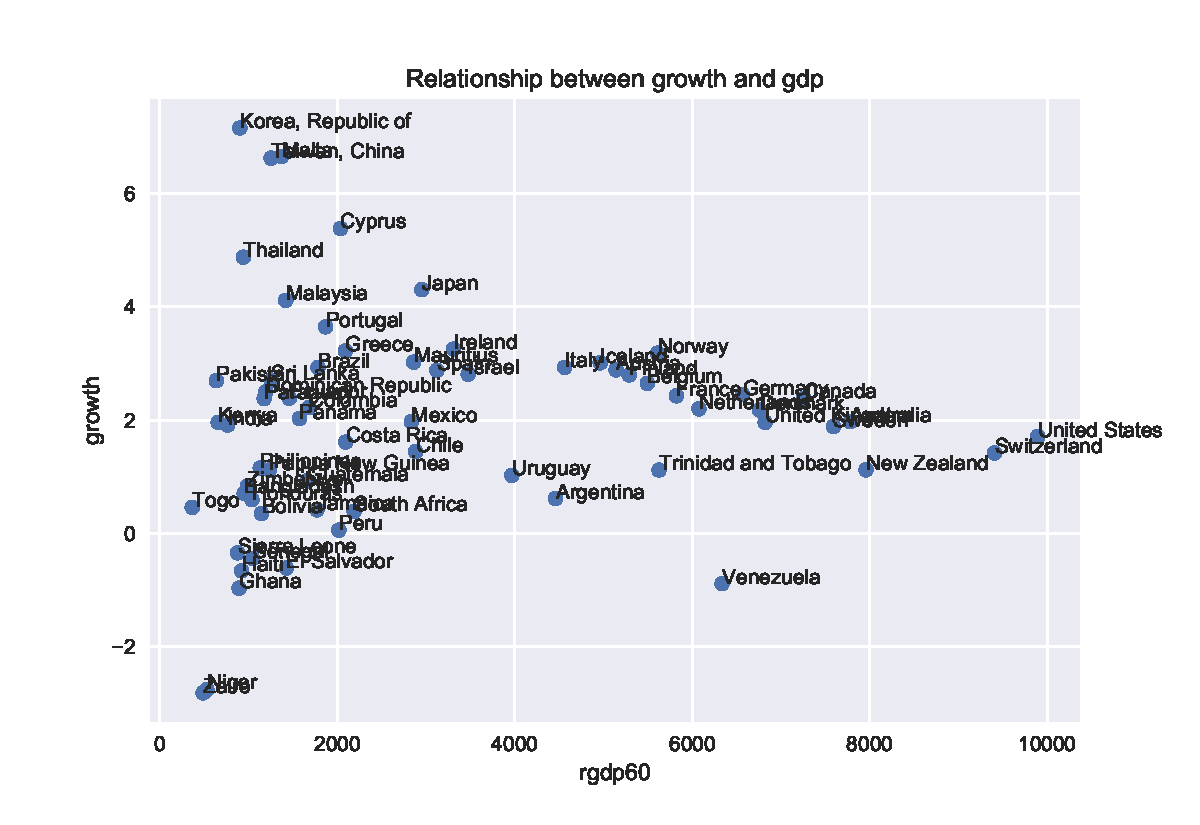
\includegraphics[width=\figwidth,height=\figheight]{GrowthGDP_fig.pdf}
 \end{frame}

\begin{frame}\frametitle{Example: Education and GDP}
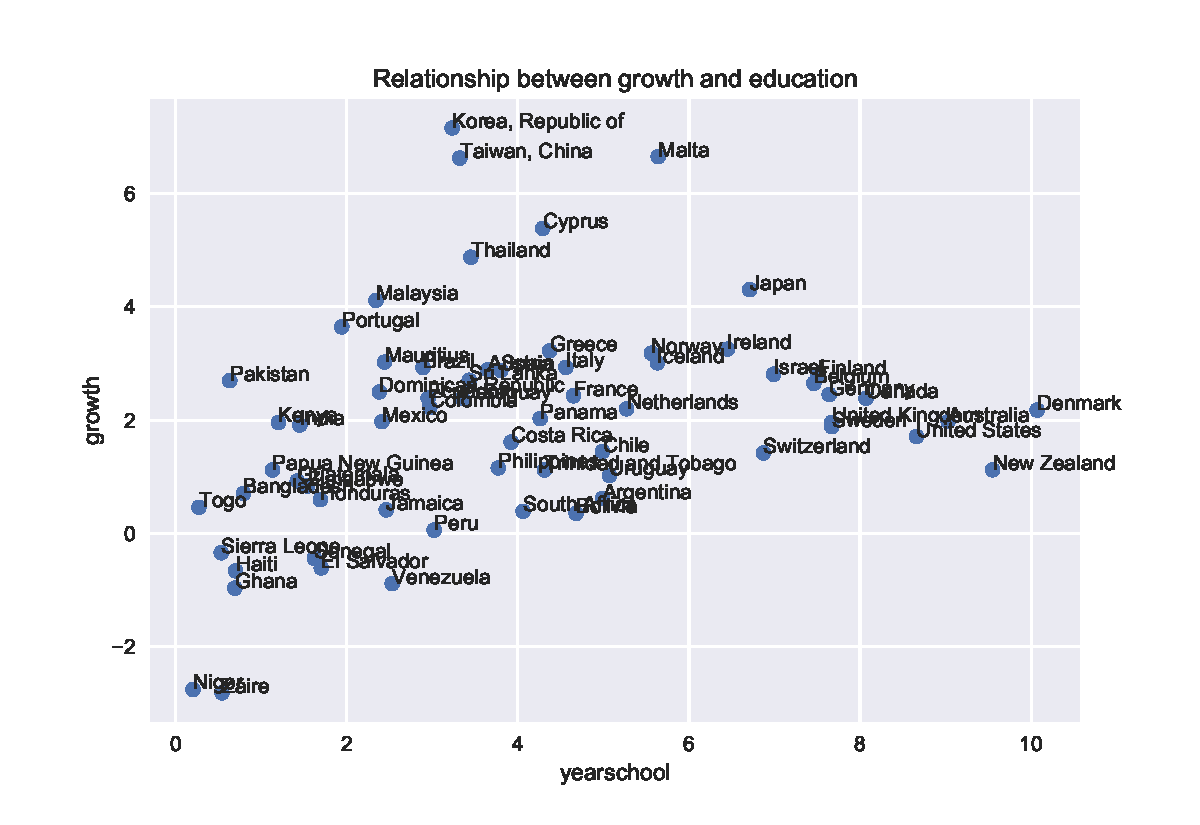
\includegraphics[width=\figwidth,height=\figheight]{GrowthSchool_fig.pdf}
\end{frame}


\section{Conditional expectation function}

\begin{frame}[allowframebreaks]
  \frametitle{Conditional expectation function}
  \begin{itemize}
  \item One way to describe relation between two variables is a
    function, 
    \begin{align*} 
Y &= h(X) 
\end{align*}
  \item Most relationships in data are not deterministic, so look at
    average relationship,
    \begin{align*}
      Y &=  \underbrace{\Er[Y|X]}_{\equiv h(X)} + \underbrace{\left(Y
          - \Er[Y|X]\right)}_{\equiv U}  \\  
      &= \Er[Y|X] + U
    \end{align*}
  \item Note that $\Er[U] = 0$ (by definition of $U$ and
    iterated expectations)
  \item $\Er[Y|X]$ can be any function, in particular, it need not be
    linear
  \item Unrestricted $\Er[Y|X]$ hard to work with
    \begin{itemize} 
    \item Hard to estimate
    \item Hard to communicate if $X$ a vector (cannot draw graphs) 
    \end{itemize}
  \item Instead use linear regression
    \begin{itemize}
    \item Easier to estimate and communicate
    \item Tight connection to $\Er[Y|X]$
    \end{itemize}
  \end{itemize}
\end{frame}  


\section{Population regression} 
\begin{frame}[allowframebreaks]\frametitle{Population regression}
  \begin{itemize}
  \item The bivariate \alert{population regression} of $Y$ on $X$ is 
    \[ (\beta_0, \beta_1) = \argmin_{b_0,b_1} \Er[(Y - b_0 - b_1
    X)^2 ] \] 
    i.e. $\beta_0$ and $\beta_1$ are the slope and intercept that
    minimize the expected square error of $Y - (\beta_0 + \beta_1 X)$ 
  \item Calculating $\beta_0$ and $\beta_1$:
    \begin{itemize}
    \item First order conditions:
      \begin{align}
        [b_0]: 0 & =  \frac{\partial}{\partial b_0} \Er[(Y - b_0 - b_1
        X)^2 ] \notag \\
         &=  \Er\left[\frac{\partial}{\partial b_0}  (Y - b_0 - b_1 X)^2 \right]
         \notag \\
        &=  \Er\left[ -2(Y - \beta_0 - \beta_1 X) \right] \label{b0}
      \end{align}
      and
      \begin{align}
        [b_1]:  0 &=  \frac{\partial}{\partial b_1} \Er[(Y - b_0 - b_1
        X)^2 ] \notag \\
         &=  \Er\left[\frac{\partial}{\partial b_1}  (Y - b_0 - b_1 X)^2 \right]
        \notag \\
        &=  \Er\left[ -2(Y - \beta_0 - \beta_1 X)X \right] \label{b1}
      \end{align}
    \item (\ref{b0}) rearranged gives $\beta_0 = \Er[Y] - \beta_1
      \Er[X]$
    \item Substituting into (\ref{b1})
      \begin{align*}
        0 &=  \Er\left[ X(-Y + \Er[Y] - \beta_1 \Er[X] + \beta_1 X) \right] \\
        &=  \Er\left[X(-Y + \Er[Y])\right] + \beta_1\Er\left[X(X -
          \Er[X])\right] \\
        &=  -\Cov(X,Y) + \beta_1 \Var(X) \\
        \beta_1 &=  \frac{\Cov(X,Y)}{\Var(X)}
      \end{align*}
    \end{itemize}
  \item \alert{$\beta_1 = \frac{\Cov(X,Y)}{\Var(X)}$, $\beta_0 = \Er[Y] - \beta_1
      \Er[X]$}
  \end{itemize}
\end{frame}

\begin{frame}\frametitle{Population regression approximates
    $\Er[Y|X]$}
  \begin{lemma} \label{lem:regapprox}
    The population regression is the minimal mean square error linear
    approximation to the conditional expectation function, i.e.\
    {\footnotesize{
        \begin{align*}
      \underbrace{\argmin_{b_0, b_1} \Er\left[\left(Y-(b_0 + b_1
          X) \right)^2\right]}_{\text{population regression}} =
      \argmin_{b_0, b_1} \underbrace{\Er_X\left[\left(\Er[Y|X] - (b_0 + b_1
          X)\right)^2\right]}_{\text{MSE of linear approximation to $\Er[Y|X]$}}
    \end{align*}
  }}
  \end{lemma}
  
  \begin{corollary} 
    If $\Er[Y|X] = c + m X$, then the population regression of $Y$ on
    $X$ equals $\Er[Y|X]$, i.e. $\beta_0 = c$ and $\beta_1 = m$
  \end{corollary}
\end{frame}

\begin{frame}[shrink]\frametitle{Proof}
  \begin{proof}
    \begin{itemize}
    \item Let $b^*_0, b^*_1$ be minimizers of MSE of approximation to $\Er[Y|X]$
    \item Same steps as in population regression formula gives
      \[ 0 = \Er\left[ -2(\Er[Y|X] - b^*_0 - b^*_1 X) \right]  \]
      and
      \[ 0 = \Er\left[ -2(\Er[Y|X] - b^*_0 - b^*_1 X)X \right]  \]
    \item Rearranging and combining,
      \begin{align*}
        b_0^* = \Er[\Er[Y|X]] - b_1^* \Er[X] = \Er[Y] - b_1^* \Er[X]
      \end{align*}
      and
      \begin{align*}
        0 = & \Er\left[ X(-\Er[Y|X] + \Er[Y] + b^*_1 \Er[X] - b^*_1 X) \right] \\
        = & \Er\left[X(-\Er[Y|X] + \Er[Y])\right] + b^*_1\Er\left[X(X -
          \Er[X])\right] \\
        = & -\Cov(X,Y) + b^*_1 \Var(X) \\
        b^*_1 = & \frac{\Cov(X,Y)}{\Var(X)}      
      \end{align*}
    \end{itemize}
  \end{proof}
\end{frame}

\subsection{Interpretation}
\begin{frame} \frametitle{Regression interpretation}
  \begin{itemize}
  \item Regression $=$ best linear approximation to $\Er[Y|X]$
  \item $\beta_0 \approx \Er[Y|X=0]$
  \item $\beta_1 \approx \frac{d}{dx} \Er[Y|X] \approx$ change in average
    $Y$ per unit change in $X$
  \item Not necessarily a causal relationship (usually not)
  \item Always can be viewed as description of data
  \end{itemize}
\end{frame}

\begin{frame}\frametitle{Regression with binary $X$}
  
      \begin{itemize}
      \item Suppose $X$ is binary (i.e. can only be $0$ or $1$)
      \item We know $\beta_0 + \beta_1 X = $ best linear approximation to
        $\Er[Y|X]$ 
      \item $X$ only takes two values,

        \begin{itemize}
        \item $\beta_0 = \Er[Y|X=0]$
        \item $\beta_0 + \beta_1 = \Er[Y|X=1]$
        \end{itemize}

      \end{itemize}
    
\end{frame}

\section{Sample regression}
\begin{frame}[allowframebreaks] \frametitle{Sample regression}
  \begin{itemize}
  \item Have sample of observations: $\{ (Y_i, X_i) \}_{i=1}^N$ 
  \item The \alert{sample regression} (or when unambiguous just
    ``regression'') of $Y$ on $X$ is 
    \[ (\hat{\beta}_0, \hat{\beta}_1) = \argmin_{b_0,b_1}
    \frac{1}{N}\sum_{i=1}^N (Y_i - b_0 - b_1 X_i)^2 \] 
    i.e. $\hat{\beta}_0$ and $\hat{\beta}_1$ are the slope and intercept that
    minimize the sum of squared errors, $(Y_i - (\hat{\beta}_0 + \hat{\beta}_1 X_i))^2$ 
    \begin{itemize}
    \item Same as population regression but with sample average
      instead of expectation
    \end{itemize}
  \item Same calculation as for population regression would show
    \[ \hat{\beta}_1 = \frac{\widehat{\Cov}(X,Y)}{\widehat{\Var(X)}} =
    \frac{\frac{1}{N} \sum_{i=1}^N (X_i -\bar{N})(Y_i - \bar{Y})}
    {\frac{1}{N} \sum_{i=1}^N (X_i - \bar{X})^2} \]
    and 
    \[ \hat{\beta}_0 = \bar{Y} - \hat{\beta}_1 \bar{X} \]
 

\framebreak

\item Since $\hat{\beta}_1$ and $\hat{\beta}_0$ come from minimizing a sum
of squares, they are called the ordinary least squares estimates, or
OLS for short. 

\item The formulas for $\hat{\beta}_1$ and $\hat{\beta}_0$ come from the
first order conditions.  

\item These estimators minimize the sum of squared
differences between the regression line and the observed $Y_i$, 
\[ (\hat{\beta}_0, \hat{\beta}_1) = \argmin_{b_0,b_1}
\frac{1}{N}\sum_{i=1}^N (Y_i - b_0 - b_1 X_i)^2. \] 
The first order condition for $\hat{\beta}_0$ is:
\begin{align*}
  0 &=  \frac{1}{N} \sumin 2(Y_i - \hat{\beta}_0 - \hat{\beta}_1 X_i ) 
\end{align*}
which can be rearranged to get
\begin{align*}
  \hat{\beta}_0 &=  \frac{1}{N} \left(\sumin Y_i - \hat{\beta}_1 X_i
  \right) \\
  \hat{\beta}_0 &=  \bar{Y} - \hat{\beta}_1 \bar{N}.
\end{align*}
The first order condition for $\hat{\beta}_1$ is: 
\begin{align*}
  0 &=  \frac{1}{N} \sumin 2X_i (Y_i - \hat{\beta}_0 - \hat{\beta}_1 X_i ).
\end{align*}
Substituting in the previous expression for $\hat{\beta}_0$ gives
\begin{align*}
  0 &=  \frac{1}{N} \sumin 2 X_i (Y_i - \bar{Y} + \hat{\beta}_1 \bar{X} - \hat{\beta}_1 X_i ). 
\end{align*}
Rearranging to solve for $\hat{\beta}_1$:
\begin{align*}
  \hat{\beta}_1 \sumin X_i(X_i - \bar{X}) &=  \sumin X_i (Y_i -
  \bar{Y}) \\
  \hat{\beta}_1 &=  \frac{\sumin X_i (Y_i - \bar{Y})}{ X_i (X_i -
    \bar{X}) } = \frac{\sumin (X_i - \bar{X}) (Y_i - \bar{Y})}{ (X_i -
    \bar{X})^2 }.
\end{align*}
 \end{itemize}
\end{frame}

\begin{frame}[allowframebreaks]
  \frametitle{Sample regression}
  \begin{itemize}
  \item Sample regression is an estimator for the population
    regression
  \item Given an estimator we should ask:
    \begin{itemize}
    \item Unbiased?
    \item Variance?
    \item Consistent?
    \item Asymptotically normal?
    \end{itemize}
  \item We will address these questions in the next week or two  
  \end{itemize}
\end{frame}

\begin{frame}[allowframebreaks]
  \frametitle{True linear model approach to regression}
  \begin{itemize}
  \item Most authors (like Wooldridge) introduce regression by
    starting with a linear model for $Y$:
    \[ Y = \alpha_0 + \alpha_1 X + \underbrace{U}_{\text{unobserved}} \] 
    with $\Er[U X] = 0$
    \begin{itemize}
    \item Perspective: model $=$ true description of data generating
      process 
    \end{itemize}
  \item Implications:
    \begin{itemize}
    \item Population regression coefficients $=$ model coefficients,
      i.e. $\beta_0 = \alpha_0$ and $\beta_1 = \alpha_1$
    \item Conditional expectation function is linear 
      \[ \Er[Y|X] = \alpha_0 + \alpha_1 X \]
    \item $\beta_1=\alpha_1$ has causal interpretation as long as we
      believe $\Er[U X] = 0$
    \item Easier to discuss causality
    \item Easier to derive statistical properties
    \end{itemize}
  \end{itemize}
\end{frame}

\begin{frame}[allowframebreaks]
  \frametitle{Problems with true linear models}
  \begin{itemize}
  \item Usually do not believe models are linear, e.g.\ no economic
    theory that says the following should be linear:
    \begin{enumerate}
    \item $\log (wage_i) = \beta_0 + \beta_1 (educ_i) + U_i$
    \item $\log q_t = \beta_0 + \beta_1 \log p_t + U_t$
    \end{enumerate}
  \item Usually do not believe error terms are uncorrelated with
    covariates, e.g.\
    \begin{enumerate}
    \item Need $\Er[U_i educ_i]=0$, but $U_i$ probably includes IQ,
      propensity to work hard, etc, which should be correlated with
      education 
    \item Is it supposed to be demand or supply? Either case, changes
      in $q_t$ from $U_t$ generally also change equilibrium $p_t$, so
      $\Er[\log p_t U_t ] \neq 0$
    \end{enumerate}
  \item Viewing regression as best linear approximation to $\Er[Y|X]$
    makes it clear what regression tells you about the data even if
    the true model is not linear and does not have $\Er[XU]=0$
  \end{itemize}
\end{frame}

\part{Properties of regression}

\frame{\partpage}
\begin{frame}
  \tableofcontents  
\end{frame}

\section{Fitted value and residuals}

\begin{frame}[allowframebreaks]
  \frametitle{Fitted values and residuals}
  \begin{itemize}
  \item These algebraic identities about fitted values and residuals are
things that we will use repeatedly later. 
\item I would not recommend spending time trying to memorize these. 
\item The important ones will come
up repeatedly and you will remember them without any special
effort. 
\item The first time we use these identities, we will go through how
to get them again. We may even go through them yet again the second
and third time we use them. 
\item Eventually we will use some of these
identities so often that you will either be able to quickly derive
them or just remember them.
 \item \alert{Fitted values}: 
    \[ \hat{Y}_i = \hat{\beta}_0 +
    \hat{\beta}_1 X_i \]
  \item \alert{Residuals}: 
    \[\hat{U}_i = Y_i - \hat{\beta}_0 -
    \hat{\beta}_1 X_i = Y_i  - \hat{Y}_i \] 
    \[ Y_i = \hat{Y}_i + \hat{U}_i \]
  \item Sample mean of residuals $=0$
    \begin{itemize}
    \item First order condition for $\hat{\beta}_0$,
      \begin{align*}
        0 = &\avg (Y_i - \hat{\beta}_0 - \hat{\beta}_1
        X_i) \\ 
        0 = & \avg \hat{U}_i 
      \end{align*}
    \end{itemize}
  \item Sample covariance of $X$ and $\hat{U}$ $= 0$
    \begin{itemize}
    \item First order condition for $\hat{\beta}_1$,
      \begin{align*}
        0 = &\avg (Y_i - \hat{\beta}_0 - \hat{\beta}_1
        X_i)X_i \\ 
        0 = & \avg \hat{U}_i X_i
      \end{align*}
    \end{itemize}
  \item Sample mean of $\hat{Y}_i = \bar{Y} = \hat{\beta}_0 +
    \hat{\beta}_1 \bar{X}$ 
    \begin{align*}
      \avg Y_i = & \avg \hat{Y}_i + \hat{U}_i \\
      = & \avg \hat{Y}_i \\
      = & \avg  \hat{\beta}_0 + \hat{\beta}_1 X_i \\
      = & \hat{\beta}_0 + \hat{\beta}_1 \bar{X}
    \end{align*}
  \item Sample covariance of $Y$ and $\hat{U}$ = sample
    variance of $\hat{U}$:
    \begin{align*}
      \avg Y_i (\hat{U}_i - \bar{\hat{U}}) = & \avg Y_i
      \hat{U}_i \\
      = & \avg (\hat{\beta}_0 + \hat{\beta}_1 X_i +
      \hat{U}_i)\hat{U}_i \\
      = & \hat{\beta}_0 \avg \hat{U}_i + \beta_1 \avg X_i
      \hat{U}_i + \avg \hat{U}_i^2 \\
      = & \avg \hat{U}_i^2 
    \end{align*}
\end{itemize}
\end{frame}

\begin{frame}[allowframebreaks]
  \frametitle{$R^2$}
  \begin{itemize}
  \item Decompose $Y_i$
    \[ Y_i = \hat{Y}_i + \hat{U}_i \]
  \item Total sum of squares $=$ explained sum of squares $+$ sum of
    squared residuals
    \[ \underbrace{\avg (Y_i - \bar{Y})^2}_{SST} =
    \underbrace{\avg (\hat{Y}_i - \bar{Y})^2}_{SSE} +
    \underbrace{\avg \hat{U}_i^2}_{SSR} \]
  \item \alert{R-squared}: fraction of sample variation in $Y$ that is
    explained by $X$
    \[ R^2 = \frac{SSE}{SST} = 1 - \frac{SSR}{SST} =o
    \widehat{\corr}(Y,\hat{Y}) \]
    \begin{itemize}
    \item $0 \leq R^2 \leq 1$
    \item If all data on regression line, then $R^2 = 1$
    \item Magnitude of $R^2$ does not have direct bearing on economic
      importance of a regression
    \end{itemize}
  \end{itemize}
\end{frame}

\section{Statistical properties}

\subsection{Unbiased}
\begin{frame}[allowframebreaks]
  \frametitle{Unbiased}
  \begin{itemize}
  \item $\Er[\hat{\beta}] = ?$
  \item Assume:
    \begin{enumerate}
    \item[SLR.1]\label{s1} (linear model) $ Y_i = \beta_0 + \beta_1
      X_i + U_i $
    \item[SLR.2]\label{s2} (independence) $\{(X_i,Y_i)\}_{i=1}^N$ is independent random
      sample
    \item[SLR.3]\label{s3} (rank condition) $\widehat{\Var}(X) > 0$
    \item[SLR.4]\label{s4} (exogeneity) $\Er[U | X] = 0$
    \end{enumerate}
  \item Then, $\Er[\hat{\beta}_1] = \beta_1$ and $\Er[\hat{\beta}_0] = \beta_0$
\item It is more important to understand the meaning of these four
assumptions (discussed below) than the proof that regression is
unbiased.    
\end{itemize}
\end{frame}

\begin{frame}[shrink]
\begin{proof}[Regression is unbiased]
  We need to calculate $\Er[\hat{\beta}]$. First, substitute in the
  formula for $\hat{\beta}$.
  \begin{align*}
    \Er[\hat{\beta}_1] = & \Er\left[ \frac{\sumin (X_i - \bar{X}) Y_i
      }{\sumin (X_i - \bar{X})X } \right] 
  \end{align*}
  Next, substitute in the model for $Y_i$, $Y_i = \beta_0 + \beta_1
  X_i + U_i$, 
  \begin{align*}
    \Er[\hat{\beta}_1] = & \Er\left[ \frac{\sumin (X_i - \bar{X}) (\beta_0 + \beta_1
  X_i + U_i)
      }{\sumin (X_i - \bar{X})X } \right] \\
    & \text{ rearrange } \\
    = & \Er\left[ \frac{ \overbrace{\sumin X_i - \bar{X}}^{=0}}{\sumin
        (X_i - \bar{X})X } \beta_0 + \overbrace{\left(\frac{\sumin (X_i - \bar{X})
            X_i}{\sumin (X_i - \bar{X})X }\right)}^{=1} \beta_1 +
      \frac{\sumin (X_i - \bar{X})U_i} {\sumin (X_i - \bar{X})X }
    \right] \\
    & \text{ use linearity of expectation } \\ 
    = & \beta_1 + \Er\left[ \frac{\sumin (X_i - \bar{x})U_i} {\sumin (X_i - \bar{X})X }
    \right] \\
    & \text{ use iterated expectations } \\
    = & \beta_1 + \Er_X\left[ \Er_{U|X}\left[\left. \frac{\sumin (X_i -
            \bar{X})U_i} {\sumin (X_i - \bar{X})X} \right\vert X_1,
        X_2, ..., X_n \right]\right] \\
    & \text{ conditional on $X_1, ..., X_n$, $X_i$ is constant} \\
    = & \beta_1 + \Er_X\left[ \frac{\sumin (X_i -
        \bar{X})\Er[U_i|X_1, ..., X_n]} {\sumin (X_i -
        \bar{X})X} \right] \\
    & \text{ independent observations implies $\Er[U_i|X_1, ...,
      X_n] = \Er[U_i | X_i]$ } \\
    = & \beta_1 + \Er_X\left[ \frac{\sumin (X_i -
        \bar{X})\Er[U_i|X_i]} {\sumin (X_i - \bar{X})X} \right] \\
    & \text{ exogeneity assumption says that $\Er[U_i | X_i] =
      0$.} \\ 
    = & \beta_1
  \end{align*}
\end{proof}
\end{frame}

\begin{frame}
\begin{itemize}
\item Note that the first few steps of the above proof showed that 
\begin{align*}
  \hat{\beta}_1 = \beta_1 + \frac{\sumin (X_i - \bar{X})
U_i}{\sumin (X_i - \bar{X})^2}. 
\end{align*}

\item This is a very useful expression that can be used as a starting point
for calculating the variance of $\hat{\beta}_1$, and thinking about
what happens if exogeneity fails and $\Er[U|X] \neq 0$.
\end{itemize}
\end{frame}



\subsection{Variance}

\begin{frame}[allowframebreaks]
  \frametitle{Variance}
  \begin{itemize}
  \item $\Var(\hat{\beta})?$
  \item Assume SLR.1-4 and
    \begin{enumerate}
    \item[SLR.5]\label{s5} (homoskedasticity) $\Var(U | X) =
      \sigma^2$
    \end{enumerate}
  \item Then, 
    \[ \Var(\hat{\beta}_1 | \{X_i\}_{i=1}^n ) =
    \frac{\sigma^2}{\sum_{i=1}^n (X_i - \bar{X})^2} \]
    and 
    \[ \Var(\hat{\beta}_0 | \{X_i\}_{i=1}^N ) =
    \frac{\sigma^2 \avg X_i^2 }{\sum_{i=1}^N (X_i - \bar{X})^2} \]
  
\framebreak

\item As in the proof that regression is unbiased, 
\begin{align*}
  \hat{\beta}_1 = \beta_1 + \frac{\sumin (X_i - \bar{X})
    U_i}{\sumin (X_i - \bar{X})^2}. 
\end{align*}
\item We now want to take the variance of this expression. 

\item Before doing so,
it will be useful to review some properties of the variance of a sum
of random variables. 
\begin{lemma}
  Let $a$, $b$, and $c$ be constants, and $Z$ and $W$ be random
  variables. Then,
  \[ \Var(a + bZ + cW) = b^2 \Var(Z) + c^2 \Var(W) + 2 bc
  \Cov(Z,W). \]
\end{lemma}

\end{itemize}
\end{frame}

\begin{frame}[shrink]

\begin{itemize}
\item We can prove this using the definition of variance. 

\begin{proof}
  
  \begin{align*}
    \Var(a + bZ + cW) & =  \Er\left[ \left(a + bZ + cW - \Er[a + bZ + cW]\right)^2 \right] \\
    &=  \Er\left[ \left(a + bZ + cW - a - b\Er[Z] - c\Er[W]\right)^2
    \right] \\
    &=  \Er\left[\left(b(Z - \Er[Z]) + c(W - \Er[W]) \right)^2 \right]
    \\
    &=  \Er\left[ b^2 (Z - \Er[Z])^2 + 2bc (Z - \Er[Z])(W - \Er[W])\right. \\
     &\ \ \ +
      \left. c^2 (W - \Er[W])^2 \right] \\
    &=  b^2\Er\left[  (Z - \Er[Z])^2\right] + 2bc \Er\left[ (Z - \Er[Z])(W - \Er[W]) \right]\\
    &\ \ \  +
    c^2 \Er\left[ (W - \Er[W])^2 \right] \\
    &=  b^2 \Var(Z) + c^2 \Var(W) + 2 bc \Cov(Z,W)
  \end{align*}
\end{proof}
\end{itemize}
\end{frame}

\begin{frame}

\begin{itemize}
\item  Generalizing the above to the sum of more than two random variables,
we have
\begin{corollary}
  Let $a_1, ..., a_n$ be constants, and $Z_1, ..., Z_n$ be random
  variables, then,
  \[
  \Var\left( \sumin a_i Z_i \right)  = \sumin \sum_{j=1}^N a_i a_j
  \Cov(Z_i, Z_j) 
  \]
  Furthermore, if $Z_i$ and $Z_j$ are independent (or just
  uncorrelated) for $i \neq j$, then
  \[
  \Var\left( \sumin a_i Z_i \right)  = \sumin a_i^2 \Var(Z_i)
  \]
\end{corollary}

 \end{itemize}
\end{frame}

\begin{frame}[shrink]

\begin{itemize}

\item We can apply this corollary to 

\begin{align*}
  \Var(\hat{\beta}_1|x) &=  \Var\left(\left. \beta_1 + \frac{\sumin (X_i - \bar{X})
        U_i}{\sumin (X_i - \bar{X})^2} \right\vert x \right)  \\
  &=  \Var\left(\left. \sumin \underbrace{\frac{X_i - \bar{X}}{\sumin (X_i -
          \bar{X})^2}}_{a_i} \underbrace{U_i}_{Z_i} \right\vert x
  \right)
  \ \ \  \text{ using the corollary } \\
  &=  \sumin \sum_{j=1}^N \frac{X_i - \bar{X}}{\sumin (X_i -
    \bar{X})^2} \frac{x_j - \bar{X}}{\sumin (X_i -
    \bar{X})^2} \Cov(U_i, U_j | X)
  \ \ \  \text{ independence } \\
  &=  \sumin \left(\frac{X_i - \bar{X}}{\sumin X_i - \bar{X}}
  \right)^2 \Var(U_i | X) 
  \ \ \  \text{ homoskedasticity} \\
 & =  \sumin \frac{(X_i - \bar{X})^2}{\left( \sumin (X_i - \bar{X})^2
    \right)^2} \sigma_U^2 \\
 & =  \frac{\sigma_U^2}{\sumin (X_i - \bar{X})^2}.
\end{align*}
\end{itemize}
\end{frame}

\subsection{Distribution}
\begin{frame}[allowframebreaks]
  \frametitle{Distribution with normal errors}
  \begin{itemize}
  \item Assume SLR.1-SLR.5 and
    \begin{enumerate}
    \item[SLR.6] (normality) $U_i|X_i \sim N(0,\sigma^2)$
    \end{enumerate}
  \item Then $Y|X \sim N(\beta_0 + \beta_1 X, \sigma^2)$, and
    \[ \hat{\beta}_1|\{X_i\}_{i=1}^N \sim N\left(\beta_1, \frac{\sigma^2}{\sum_{i=1}^N
        (X_i - \bar{X})^2} \right) \]
  \item Even without assuming normality, the central limit theorem
    implies $\hat{\beta}$ is asymptotically normal (details in a later
    lecture)
\framebreak
  \item An important property of normal random variables is that if $Z$ and
$W$ are independent, and $Z \sim N(\mu_z, \sigma_z^2)$ and $W \sim
N(\mu_w, \sigma_w^2)$, then 
\[ a + bZ + cW \sim N(a + b \mu_z + c \mu_w, b^2 \sigma^2_z + c^2
\sigma^2_w). \]
\item  If we assume that $U_i$ is normally distributed
conditional on $X$, then since $\hat{\beta}_1$ is just a sum of the
$U_i$,\footnote{Specifically, $ \hat{\beta}_1 = \beta_1 +
  \frac{\sumin (X_i - \bar{X}) U_i}{\sumin (X_i -
    \bar{X})^2}$.}
$\hat{\beta}_1$ will also be normally distributed. 
 \end{itemize}
\end{frame}

\begin{frame}[allowframebreaks] \frametitle{Summary}
  \begin{itemize}
  \item Simple linear regression model assumptions:
    \begin{enumerate}
    \item[SLR.1] (linear model) $ Y_i = \beta_0 + \beta_1 X_i + U_i $
    \item[SLR.2] (independence) $\{(X_i,Y_i)\}_{i=1}^n$ is independent random
      sample
    \item[SLR.3] (rank condition) $\widehat{\Var}(X) > 0$
    \item[SLR.4] (exogeneity) $\Er[U | X] = 0$
    \item[SLR.5] (homoskedasticity) $\Var(U | X) =
      \sigma^2$
    \item[SLR.6] (normality) $U_i|X_i \sim N(0,\sigma^2)$
    \end{enumerate}
  \item $\hat{\beta}$ unbiased if SLR.1-SLR.4
  \item If also SLR.5, then $\Var(\hat{\beta}_1 | \{X_i\}_{i=1}^N ) =
    \frac{\sigma^2}{\sum_{i=1}^N (X_i - \bar{X})^2}$ 
  \item If also SLR.6, then $\hat{\beta}_1|\{X_i\}_{i=1}^N \sim
    N\left(\beta_1, \frac{\sigma^2}{\sum_{i=1}^N (X_i - \bar{X})^2}
    \right)$
  \end{itemize}
\end{frame}

\subsection{Discussion of assumptions}
\begin{frame}[allowframebreaks]
  \frametitle{Discussion of assumptions}
  \begin{itemize}
  \item[SLR.1] Having a linear model makes it easier to state the other
    assumptions, but we could instead start by saying let $\beta_1 =
    \frac{\Cov(X,Y)}{\Var(X)}$ and $\beta_0 = \Er[Y] - \beta_1 \Er[X]$
    be the population regression coefficients and define $U_i =
    Y_i - \beta_0 - \beta_1 X_i$
  \framebreak
\item To say whether an estimator is unbiased, we first have to define what
parameter we want to estimate. 
\item Assuming that there is a linear model
defines the parameter we want to estimate. 
\item This linear model could be
population regression, in which case, $\beta_1 = \frac{\Cov(X,Y)
}{\Var(X)}$, and by construction we must have
$\Er[XU]=0$. 
\item However, the linear model may also be motivated by economic
theory. 
\item For example, consider a Cobb-Douglass production function with
only one input, labor,
\[ Y = A L^\alpha, \] 
where $Y$ is output, $L$ is labor, and $A$ is productivity. 
\item If we take logs, then
\[ \log Y = \log A + \alpha \log L. \]
If we rearrange slightly, we get something that looks just like a
linear regression model, 
\[ \underbrace{\log Y_i}_{Y_i} = \underbrace{\Er[\log A]}_{\beta_0}
+ \underbrace{\alpha}_{\beta_1} \underbrace{\log L_i}_{X_i} +
\underbrace{(\log{A}_i - \Er[\log A])}_{U_i}. \]
\item If this is the model we want to estimate, then $U_i$ is not the
error term in the population regression. 
\item Instead $U_i$ is the
difference between the log productivity of firm $i$ and average log
productivity. 
\item It is unlikely that this $U_i$ would be
uncorrelated with $\log L_i$. 
\item More productive firms generally choose
to use more inputs, so we should suspect that $U_i$ and $\log
L_i$ are positively correlated.
 \end{itemize}
\end{frame}

\begin{frame}[allowframebreaks]
  \frametitle{Discussion of assumptions}
  \begin{itemize}
  \item[SLR.2] Independent observations is a good assumption for data
    from a simple random sample
    \begin{itemize}
    \item Common situations where it fails in
      economics are when we have a time series of observations,
      \item e.g.\ $\{(X_t,Y_t)\}_{t=1}^N$ could be unemployment and GDP of
      Canada for many different years; and clustering, 
      \item e.g.\ the data
      could be students test scores and hours studying and our sample
      consists of randomly chosen courses or schools---students in the
      same course would not be independent, but across different courses
      they might be.
    \item Still have $\Er[\hat{\beta}_1] = \beta_1$ with
      non-independent observations as long as $\Er[Un_i | X_1, ..., X_N] = 0$
    \item The variance of $\hat{\beta}_1$ will change with
      non-independent observations
    %\item
      %\href{https://bitbucket.org/paulschrimpf/econ326/src/master/notes/03/dependent.R?at=master}
      %{Simulation code}
    \end{itemize}
 
\item Independence says that knowing the values of $x_1$ and $y_1$ tells you
nothing about the distribution of $x_2$ and $y_2$ (or any other
observation).
\item  When we have cross-sectional data, this assumption
usually makes sense. 
\item In economics, we sometimes deal with time-series
data, where $(x_1,y_1)$ would be the observation of something at time
$1$ and $(x_2,y_2)$ is the observation that same thing at time $2$. In
this case, independence is unlikely to hold. 
\item Another common situation
is panel data, where we observe a sample of individuals over time, so
$(x_{it}, y_{it})$ would be what we observe from individual $i$ at
time $t$. 
\item Again, it is unlikely that these observations would be
independent over time.  
\item Later in the course, we will talk about how to
deal with non-independent observations.
\end{itemize}
\end{frame}

\begin{frame}[allowframebreaks]
  \frametitle{Discussion of assumptions}
  \begin{itemize}
  \item[SLR.3] If $\widehat{\Var}(X) = 0$, then 
    $\hat{\beta}_1$ involves dividing by $0$
    \begin{itemize}
    \item If there is no variation in $X$, then we cannot see how
      $Y$ is related to $X$
    \end{itemize}
  \end{itemize}
\end{frame}

\begin{frame}[allowframebreaks]
  \frametitle{Discussion of assumptions}
  \begin{itemize}
  \item[SLR.4] To think about mean independence of $U$ from $X$
    we should have a model motivating the regression
  \end{itemize}
  \begin{columns}[c] % align columns
    \begin{column}{.48\textwidth}
      \begin{itemize}
      \item If the model we want is just a population regression,
        then automatically $\Er[UX] = 0$, and $\Er[U|X] =
        0$ if the conditional expectation function is linear; if
        conditional expectation nonlinear maybe still a useful
        approximation       
      \end{itemize}
    \end{column}
    \begin{column}{.48\textwidth}
      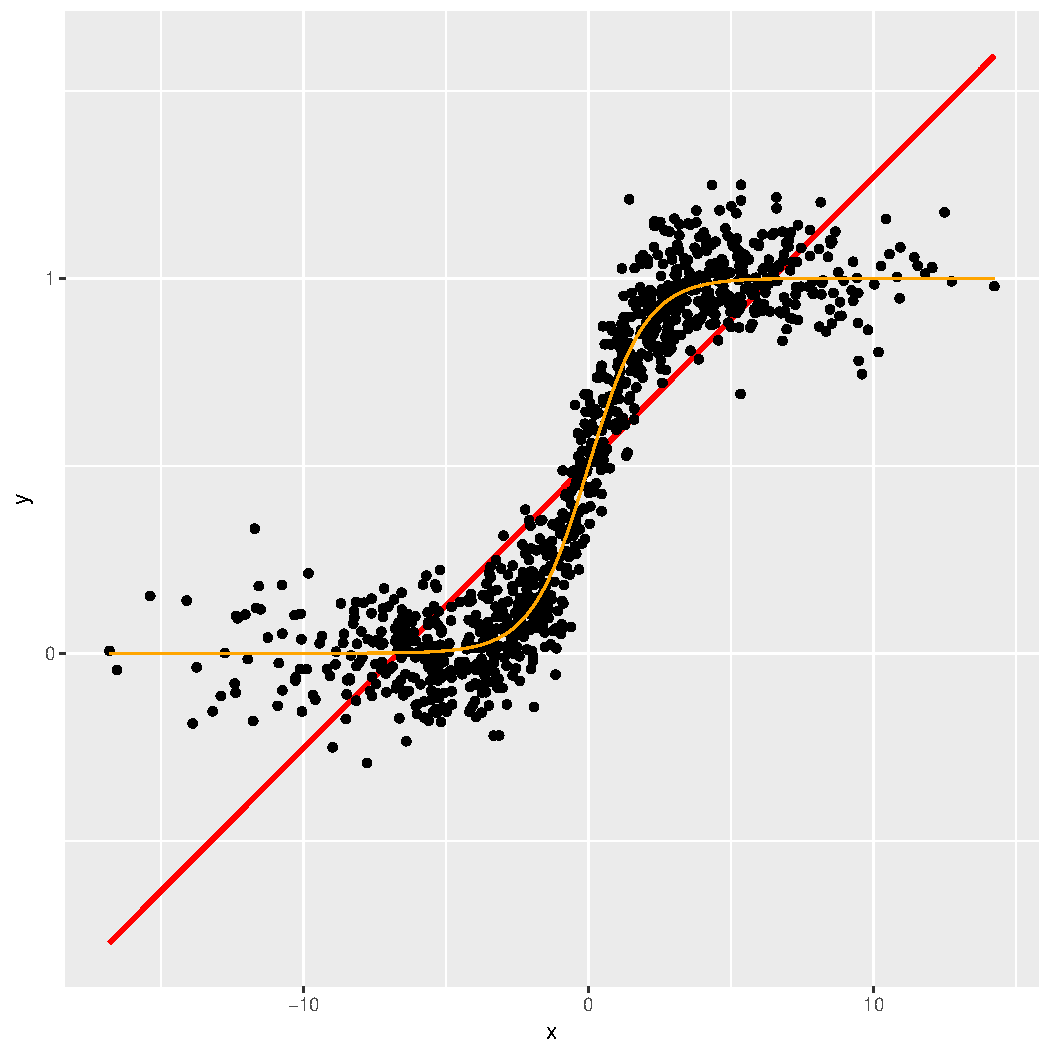
\includegraphics[width=\textwidth]{nonlinear} \\
      %\href{https://bitbucket.org/paulschrimpf/econ326/src/master/notes/03/nonlinear.R?at=master}
      %{Code}
    \end{column}
  \end{columns}
\end{frame}

\begin{frame}[allowframebreaks]
  \frametitle{Discussion of assumptions}
  \begin{itemize}
  \item[SLR.4] To think about mean independence of $U$ from $X$
    we should have a model motivating the regression
  \end{itemize}
  \begin{columns}[c] % align columns
    \begin{column}{.48\textwidth}
      \begin{itemize}
      \item If the model we want is anything else, then maybe
        $\Er[UX] \neq 0$ (and $\Er[U | X] \neq 0$), e.g.\ 
        \begin{itemize}
        \item Demand curve 
          \[ P_i = \beta_0 + \beta_1 Q_i + U_i \]
          $U_i = $ everything that affects price other than
          quantity. $Q_i$ determined in equilibrium implies
          $\Er[U_i | Q_i] \neq 0$ 
        \item $\Er[\hat{\beta}_1] \neq \beta_1$ and $\hat{\beta}_1$ does
          not tell us what we want
        \end{itemize}
      \end{itemize}
    \end{column}
    \begin{column}{.48\textwidth}
      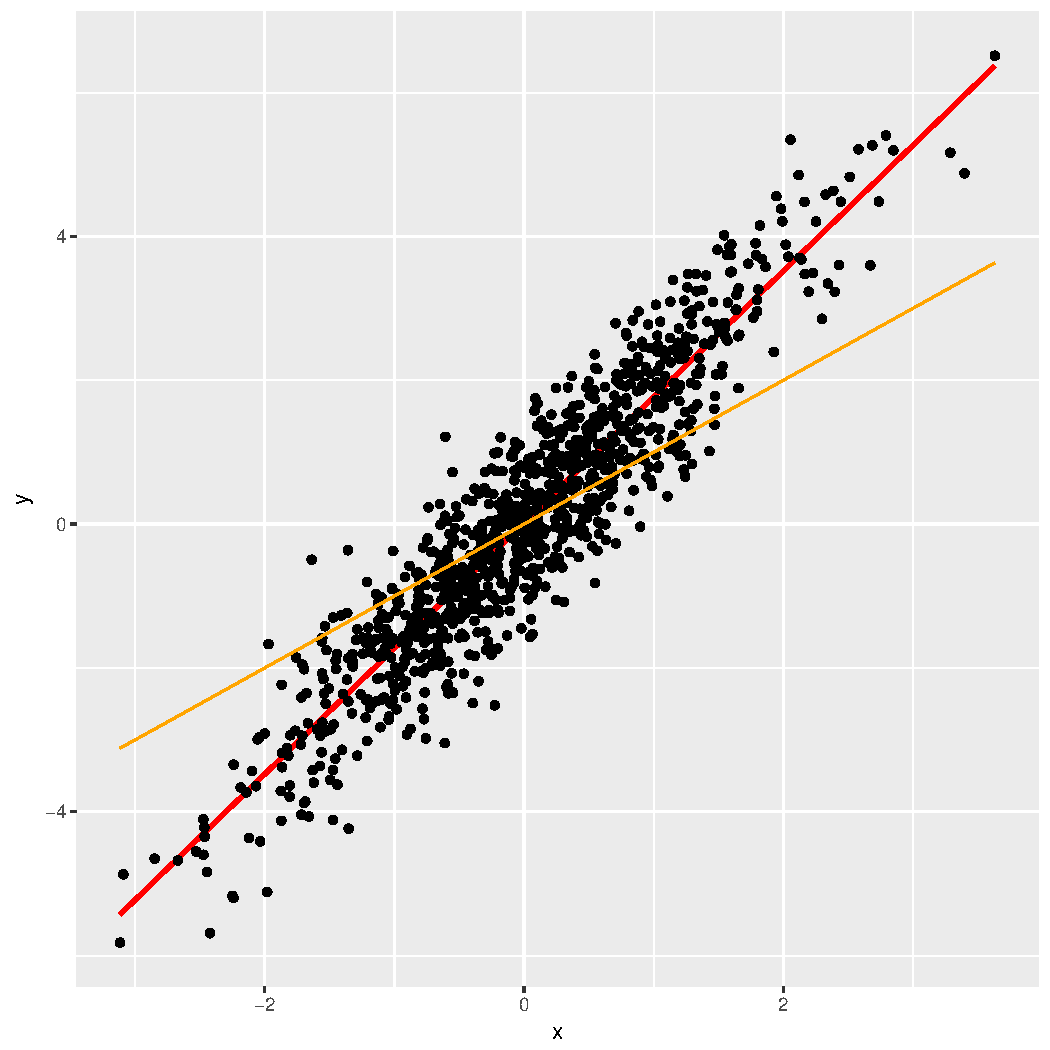
\includegraphics[width=\textwidth]{endogenous} \\
      %\href{https://bitbucket.org/paulschrimpf/econ326/src/master/notes/03/endogenous.R?at=master}
      %{Code}
    \end{column}
  \end{columns}

\framebreak

\begin{itemize}
\item Exogeneity is the most important assumption underlying
  regression. 
\item In fact, estimating any economic model using any method will involve some
kind of exogeneity assumption. 
\item By this, we mean that every estimation
method requires assuming some error term is either completely
independent of some observable ($F_{U|X}(u|x) =
F_U(u)$), mean independent of some observable
($\Er[U|X] = 0$), or at least uncorrelated with an observable
($\Er[U X] = 0$). 
\item Much of what separates good empirical work in
economics from bad is how plausible are the exogeneity
assumptions. 
\item Often, economic theory can help us decide whether or
not an exogeneity assumption is plausible. Consider the 
production function example from earlier, 
\[ \underbrace{\log Y_i}_{Y_i} = \underbrace{\Er[\log A]}_{\beta_0}
+ \underbrace{\alpha}_{\beta_1} \underbrace{\log L_i}_{X_i} +
\underbrace{(\log{A}_i - \Er[\log A])}_{U_i}. \]
\item To think about whether mean independence of the error term,
$\Er[\underbrace{(\log{A} - \Er[\log A])}|\log L]=0$, makes sense in
this model, we should think about how $L$ is determined. 
\item The firm
chooses how much labor to use. Suppose the firm faces output price $P$
and wage $W$. 
\item If the firm chooses $L$ knowing its productivity, then
the firm solves,
\begin{align*}
   \max_L P A L^\alpha - WL 
\end{align*}
The first order condition is 
\begin{align*}
  P A \alpha L^{\alpha -1} - W = & 0.
\end{align*}
If we solve for $A$, we get
\begin{align*}
  A = & \frac{W}{P \alpha } L^{1-\alpha} \\
  \log A = \log\left(\frac{W}{P \alpha }\right) + (1-\alpha) \log L
\end{align*}
so
\begin{align*}
  \Er[ \log A | \log L ] =  (1-\alpha) \log L +
  \Er\left[\left . \log\left(\frac{W}{p \alpha }\right) \right| \log L
  \right] 
\end{align*}
\item This will not be a constant unless $\alpha = 1$ and $\frac{W}{p}$ is
mean independent of $\log L$. 
\item Both of these are unlikely to
hold. 
\item Unless $\Er[ \log A | \log L ] $ is constant,
$\Er[\underbrace{(\log{A} - \Er[\log A])}|\log L] \neq 0$.  
\item Therefore,
exogeneity is not a good assumption in this model, and regression will
not give an unbiased estimate of the production function. 

\end{itemize}
\end{frame}

\begin{frame}[allowframebreaks]
  \frametitle{Discussion of assumptions}
  \begin{itemize}
  \item[SLR.5] Homoskedasticity: variance of $U$ does not
    depend on $X$ \\
    \begin{tabular}{cc} 
      \alert{Homoskedastic} & \alert{Heteroskedastic} \\ 
      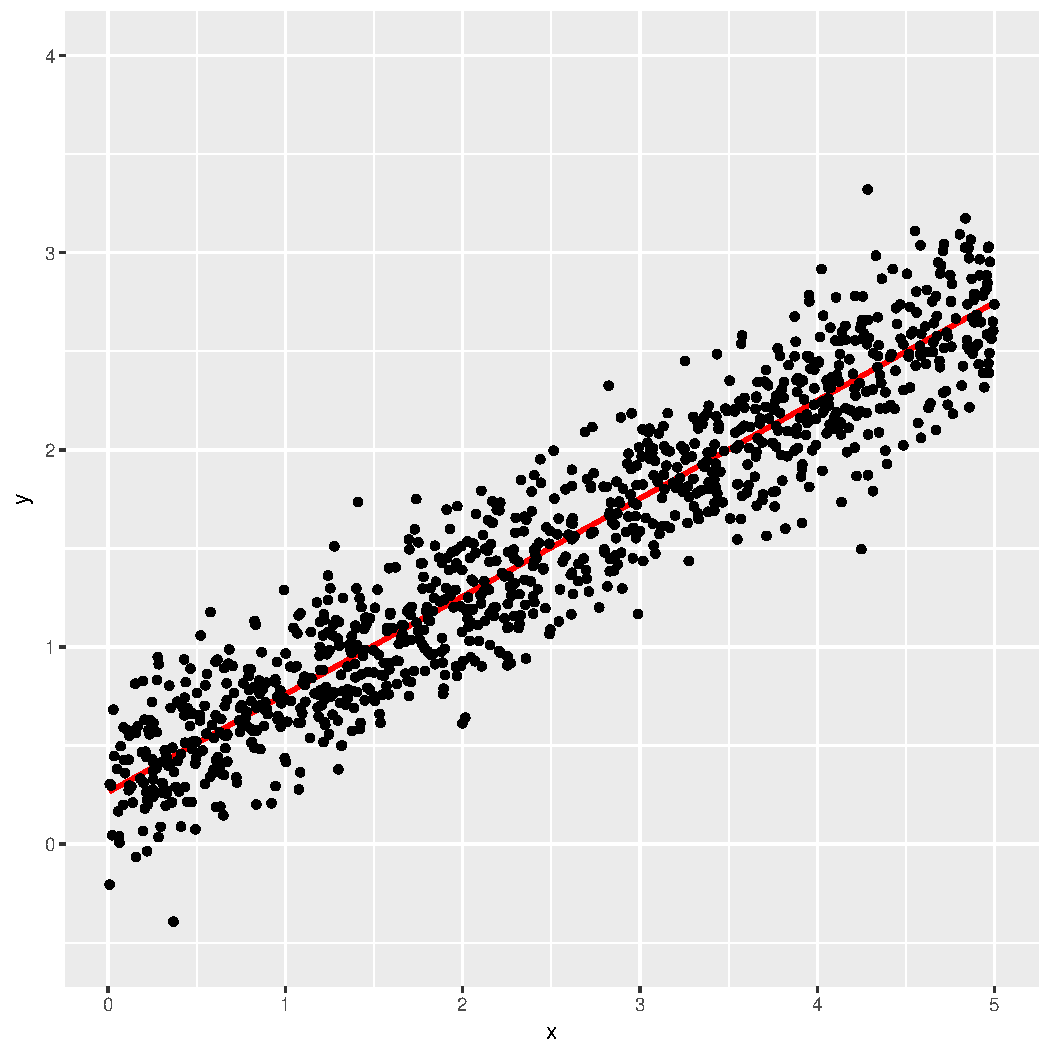
\includegraphics[width=0.4\textwidth]{homoskedastic} &
      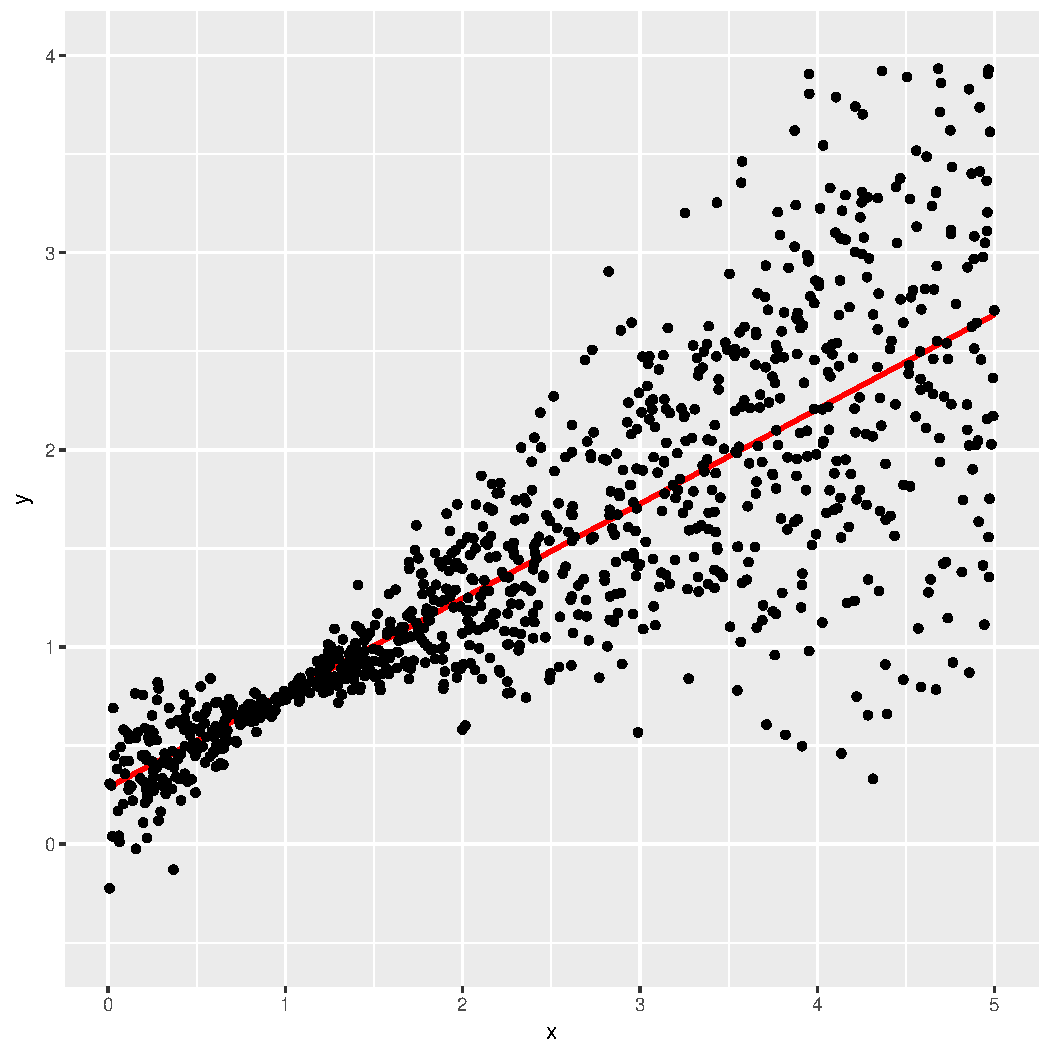
\includegraphics[width=0.4\textwidth]{heteroskedastic} 
    \end{tabular} \\
    %\href{https://bitbucket.org/paulschrimpf/econ326/src/master/notes/03/skedastic.R?at=master}
    %{Code}
    \begin{itemize}
    \item \alert{Heteroskedasticity} is when $\Var(U|X)$ varies
      with $X$
    \item If there is heteroskedasticity, the variance of
      $\hat{\beta}_1$ is different, but we can fix it 
    \item ``robust standard errors'' / ``heteroscedasticity-consistent
      (HC) standard errors'' / ``Eicker–Huber–White standard errors''
    \end{itemize}
\item Homoskedasticity is a strong assumption that is usually not very
plausible. 
\item Therefore, in practice economists almost always calculate
heteroscedasticity-robust standard errors. 
\end{itemize}
\end{frame}


\begin{frame}[allowframebreaks]
  \frametitle{Discussion of assumptions}
  \begin{itemize}
  \item[SLR.6] If $U_i|X_i \sim N$, then $\hat{\beta}_1 \sim N$
    \begin{itemize}
    \item What if $U_i$ not normally distributed?
    \item We will see that $\hat{\beta}_1$ still asymptotically normal
    %\item
     % \href{https://bitbucket.org/paulschrimpf/econ326/src/master/notes/03/reg-clt.R?at=master}
      %{Simulation}
    \end{itemize}
  \end{itemize}
\end{frame}


%\begin{frame}
 % \frametitle{Discussion of assumptions}

  %\includegraphics[width=\figwidth,height=\figheight,keepaspectratio]{beta1} 

%\end{frame}

%\begin{frame}
 % \frametitle{Discussion of assumptions}

  %\includegraphics[width=\figwidth,height=\figheight,keepaspectratio]{zbeta1} 

%\end{frame}

\begin{frame}\frametitle{Example: convergence in growth}
  \begin{itemize}
  \item Data on average growth rate from 1960-1995 for 65 countries
    along with GDP in 1960, average years of schooling in 1960, and
    other variables
  \item From
    \url{http://wps.aw.com/aw_stock_ie_2/50/13016/3332253.cw/index.html},
    originally used in \cite{beck2000}
  \item Question: has there been in convergence, i.e.\ did poorer
    countries in 1960 grow faster and catch-up?    
  \item \href{https://bitbucket.org/paulschrimpf/econ326/src/master/notes/03/growth.R?at=master} {Code}
  \end{itemize}
\end{frame}

\section{Examples}
\begin{frame}\frametitle{GDP in 1960 and growth: $\hat{\beta}_0 = 1.7958$ ,
    $\hat{\beta}_1 = 4.735e-05$. }

  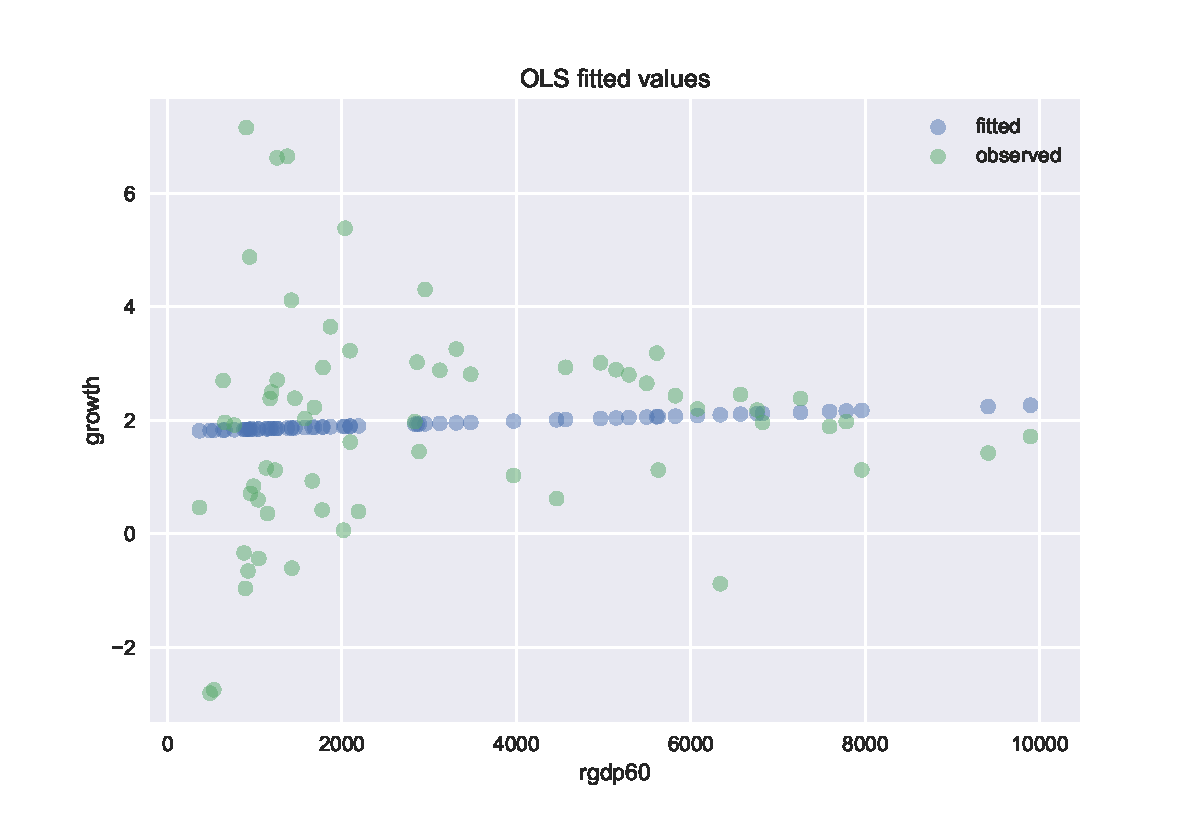
\includegraphics[width=\figwidth,height=\figheight]{lreg_GrowthGDP}   

\end{frame}

\begin{frame}\frametitle{Years of schooling in 1960 and growth: $\hat{\beta}_0 =  0.9583$ ,
    $\hat{\beta}_1 = 0.2470$.}

  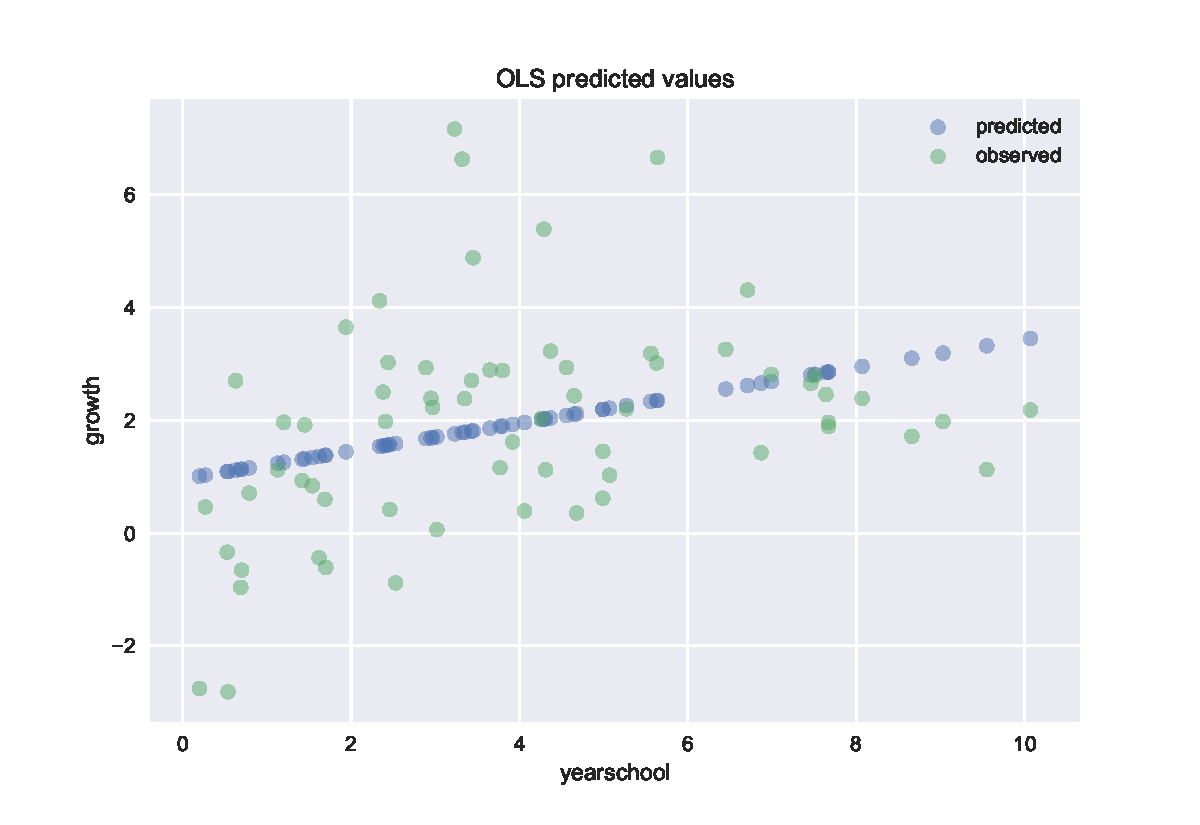
\includegraphics[width=\figwidth,height=\figheight]{lreg_GrowthSchool}   

\end{frame}

%%%%%%%%%%%%%%%%%%%%%%%%%%%%%%%%%%%%%%%%%%%%%%%%%%%%%%%%%%%%%%%%%%%%%%

\begin{frame}[allowframebreaks]
  \frametitle{References}
 \bibliographystyle{jpe}
\bibliography{../Biblio}
\end{frame}


\end{document}